  Relaciona cada tipo de termómetro con su funcionamiento.
    \begin{multicols}{2}
        \begin{choices}
            \choice \adjustbox{valign=t}{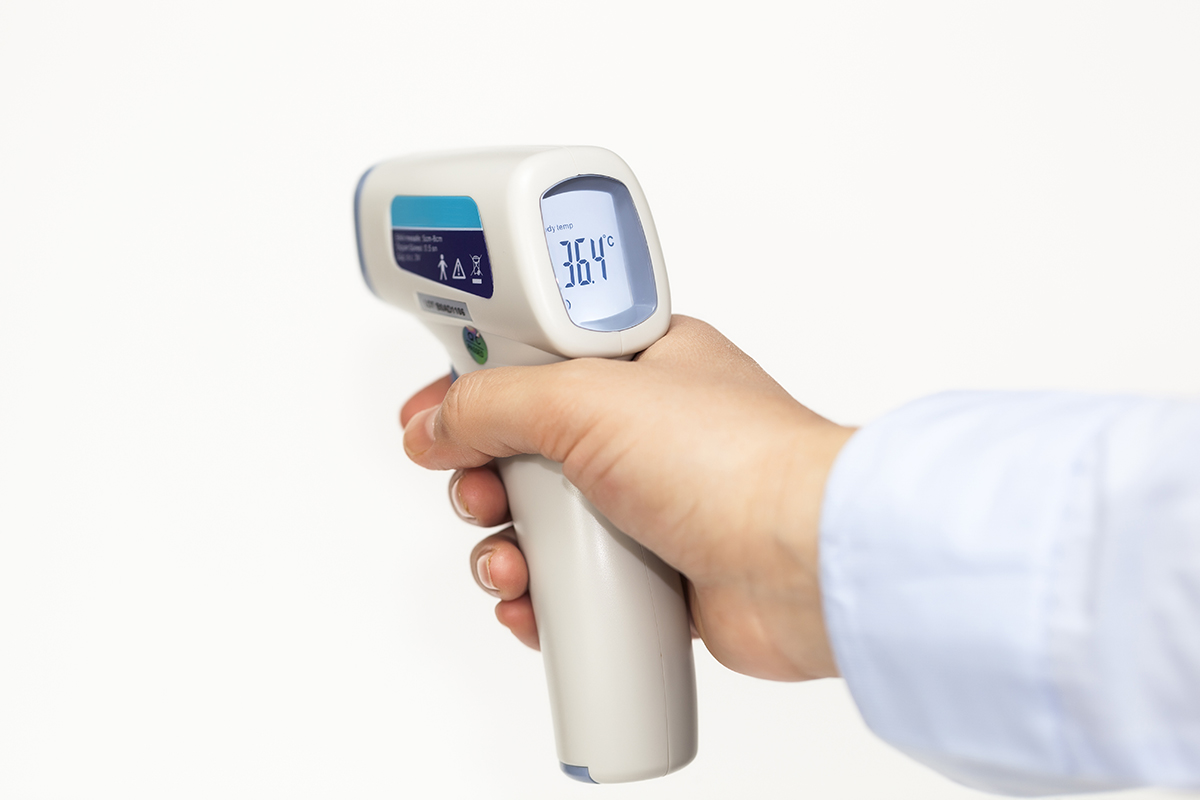
\includegraphics[width=0.25\textwidth ]{Images/SINFI_U1_AC83_IMG1.jpg} }
            $\square$
            \choice \adjustbox{valign=t}{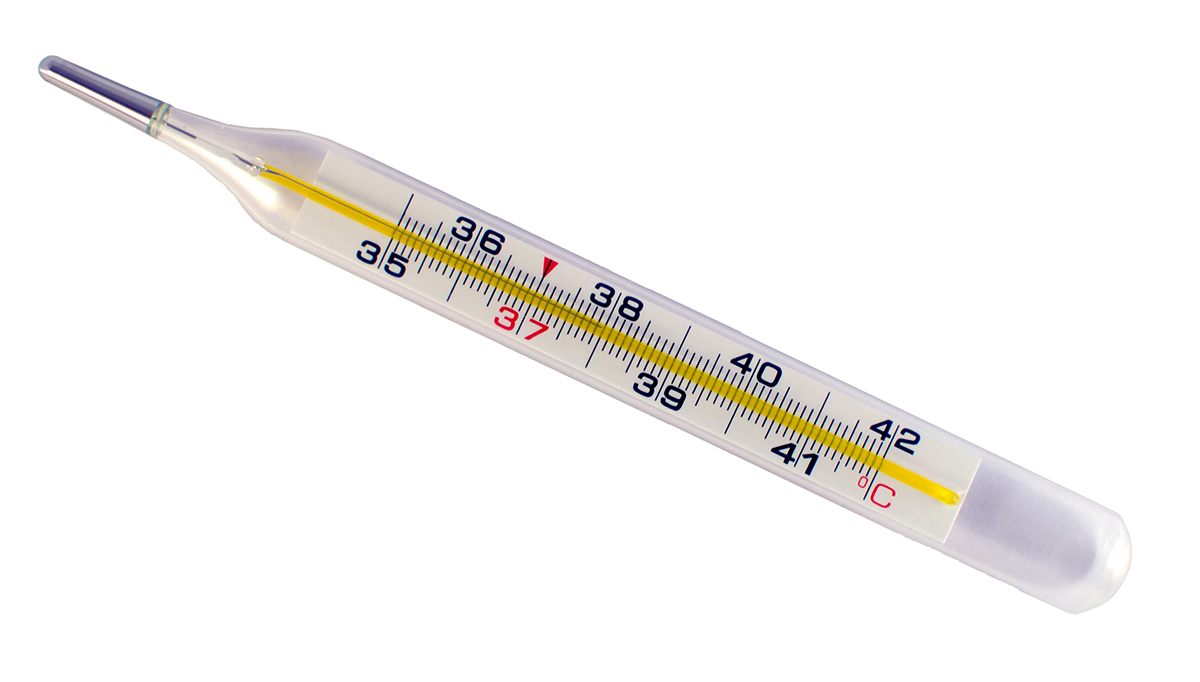
\includegraphics[width=0.25\textwidth ]{Images/SINFI_U1_AC83_IMG2.jpg} }
            $\square$
            \choice \adjustbox{valign=t}{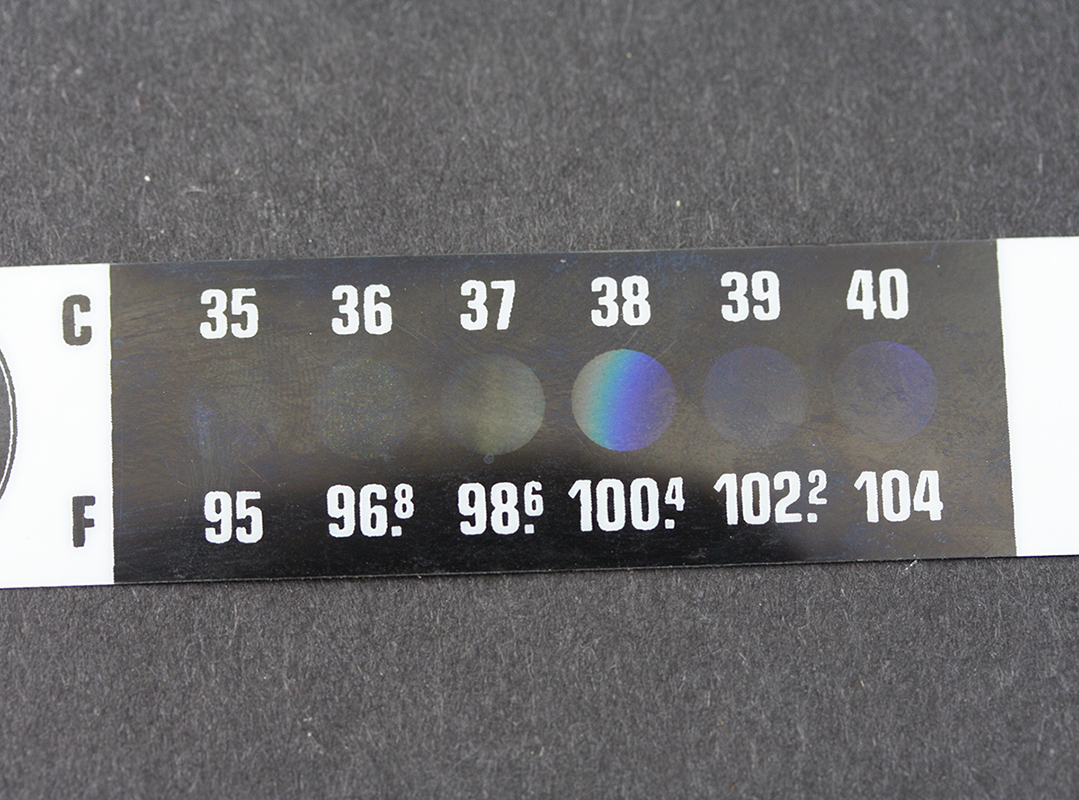
\includegraphics[width=0.25\textwidth ]{Images/SINFI_U1_AC83_IMG3.jpg} }
            $\square$
            \choice \adjustbox{valign=t}{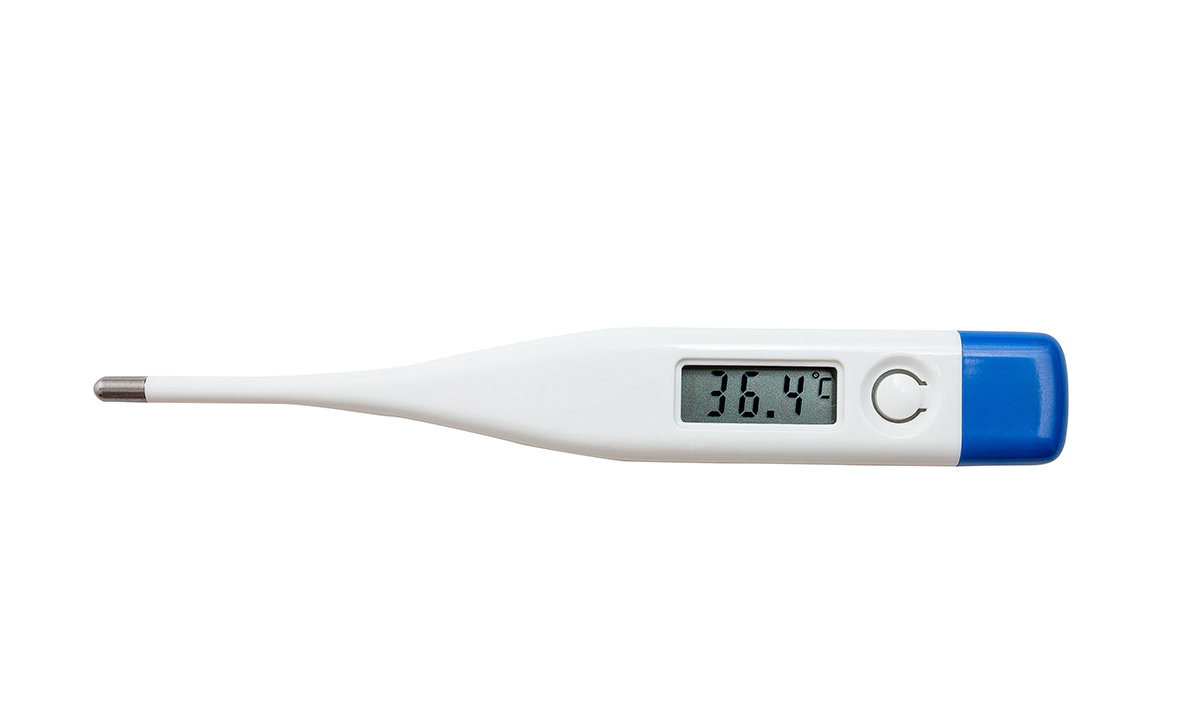
\includegraphics[width=0.25\textwidth ]{Images/SINFI_U1_AC83_IMG4.jpg} }
            $\square$
        \end{choices}
        \vspace{3cm}
        \begin{checkboxes}
            \choice Por medio de una escala, mide directamente el cambio de la longitud de una columna de ese metal líquido que varía con la temperatura.                 \vspace{1cm}
            \choice Mide la temperatura por medio de un cristal líquido que cambia de color con ésta.             \vspace{1cm}
            \choice Mide la emisión de las ondas electromagnéticas con longitud de onda entre 1 mm y 750 nm de una zona del cuerpo.
            \vspace{1cm}
            \choice Mide la temperatura por medio del cambio de voltaje en la unión de dos metales distintos que generan corrientes eléctricas que dependen de la temperatura.
            \vspace{1cm}
        \end{checkboxes}
    \end{multicols}